\documentclass[12pt,a4paper]{article}
\usepackage{inputenc}
\usepackage{amsmath}
\usepackage{amsfonts}
\usepackage{amssymb}
\usepackage{makeidx}
\usepackage{graphicx}
\usepackage{enumerate}
\usepackage{setspace}
\usepackage{longtable}
\usepackage{float}
\usepackage{hyperref}
\usepackage[framed,numbered,autolinebreaks,useliterate]{mcode}

\usepackage[left=2cm,right=2cm,top=2cm,bottom=2cm]{geometry}
\author{\vspace{-4em}N Sowmya Manojna BE17B007\vspace{-4em}}
\date{1st October 2020}
\title{\vspace{-3em}BT6270 Computational Neuroscience Assignment 1}

\usepackage{fontspec}
\setmainfont{Cambria}

\usepackage{caption}
\DeclareCaptionLabelSeparator{pipe}{ $|$ }% or $\vert$
% \captionsetup{font=small, labelfont={bf, color=blue}}
\captionsetup{font=small, labelfont={color=blue}}

\newcommand{\spa}{\vspace{1.5em}}
\newcommand{\noi}{\noindent}
\def\dul#1{\underline{\underline{#1}}}
\def\tt#1{\texttt{#1}}

\begin{document}
% \begin{titlepage} 
% 	\begin{center}
% 		\vspace{3em}
% 		\large {BT6270 Computational Neuroscience}	
% 		\vspace{10em}
		
% 		\rule{0.9\linewidth}{0.5mm} \\[0.4cm]
% 	    \large{\bfseries{Computational Neuroscience Assignment 1}} \\
% 	    \rule{0.9\linewidth}{0.5mm} \\[3 em]	
	    
% 	    N Sowmya Manojna | BE17B007\\ 
% 		Department of Biotechnology,\\
% 		Indian Institute of Technology, Madras\\    
		
% 		\vspace{5em}    
% 		
\includegraphics[scale = 0.09]{images/iitmlogo.png}

% 	\end{center}
% \end{titlepage}
\vspace{-1em}
\maketitle
\vspace{-3em}

\section{Threshold values of External Current}
The threshold currents are as follows:
\vspace{-0.5em}
\begin{itemize}
	\itemsep0em
	\item I1 = 0.03 $\mu A/mm^2$
	\item I2 = 0.06 $\mu A/mm^2$
	\item I3 = 0.45 $\mu A/mm^2$
\end{itemize}

\noi
These values were obtained with a current sampling interval of \tt{0.01}  $\mu A/mm^2$ from \tt{0} $\mu A/mm^2$ to \tt{0.6} $\mu A/mm^2$. Hence, finer thresholds are not recorded.

\section{Assumptions}
The assumptions made in the construction of the plot are as follows:
\begin{itemize}
	\itemsep0em
	\item The voltage threshold of a peak is set to \tt{10mV}. All voltage peaks greater than \tt{10mV} are considered in the spike count.
	\item Input current (\tt{I1}) at which spiking occurs is calculated by identifying the current where the number of spikes first becomes non zero.
	\item The current \tt{I2} is calculated by identifying the current at which  the number of spikes increases by more than 4 in the next current instant.
	\item The current \tt{I3} is calculated by identifying the current at which  the number of spikes decreases by more than 2 in the next current instant.
\end{itemize}

\section{Plot}
\vspace{-1em}
\begin{figure}[H]
	\centering
	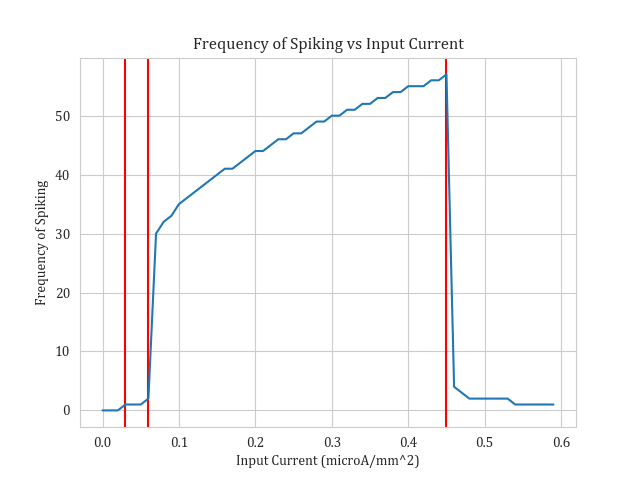
\includegraphics[scale=0.6]{images/frequency.png}
	\caption{The change in frequency of firing as a function of Input current. The number of iterations performed for each current instance: $5(10^4)$. The red vertical bars indicate the current thresholds - \tt{I1, I2 \& I3} respectively (and in the left to right order).}
\end{figure}

	% \begin{figure}[H]
	% 	\centering
	% 	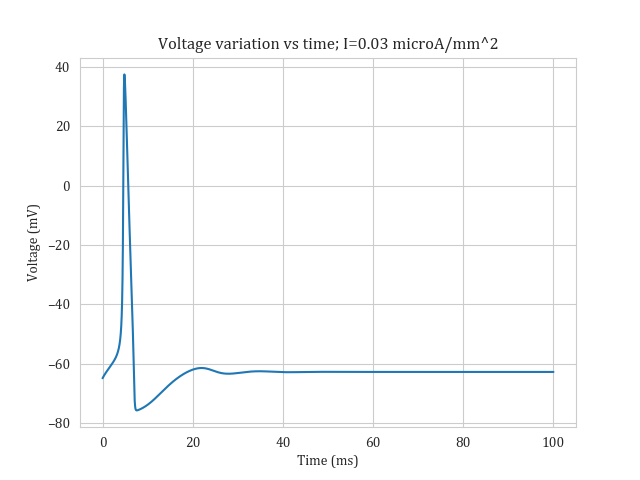
\includegraphics[scale=0.6]{images/small_i_v.png}
	% 	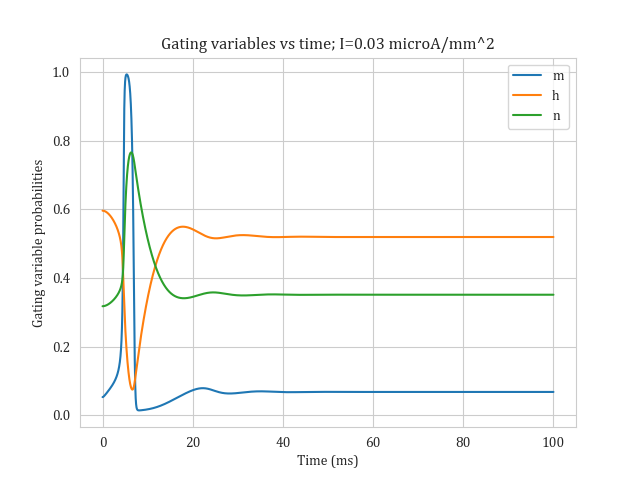
\includegraphics[scale=0.6]{images/small_i_gating.png}
	% 	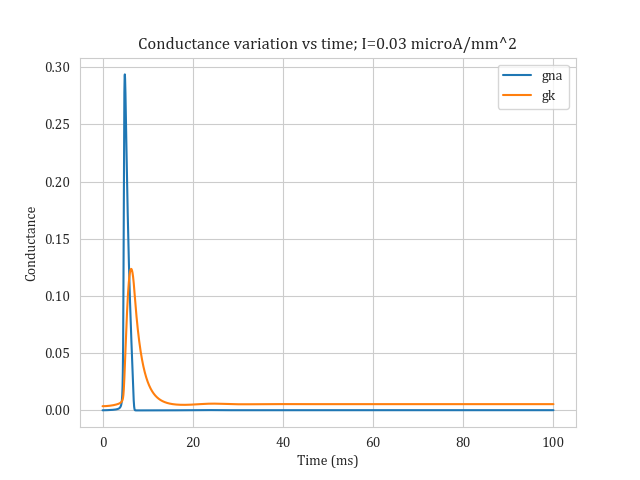
\includegraphics[scale=0.6]{images/small_i_conductance.png}
	% 	\caption{Variation of Voltage, Gating variables and Conductance at current instant \tt{I1}. A single voltage spike is observed. Number of iterations performed: $10^4$}
	% \end{figure}

	% \begin{figure}[H]
	% 	\centering
	% 	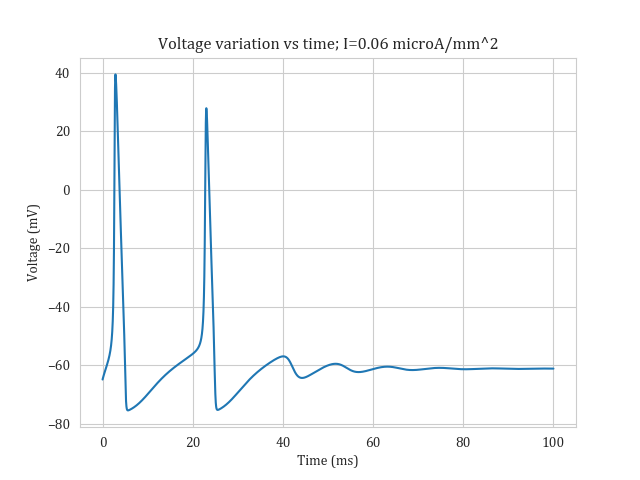
\includegraphics[scale=0.6]{images/finite_v.png}
	% 	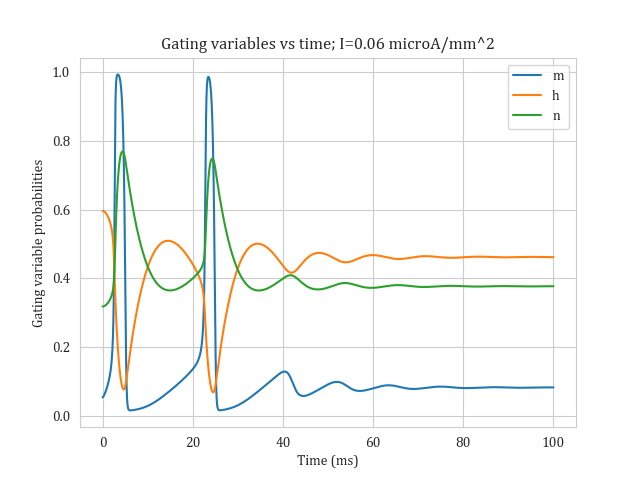
\includegraphics[scale=0.6]{images/finite_gating.png}
	% 	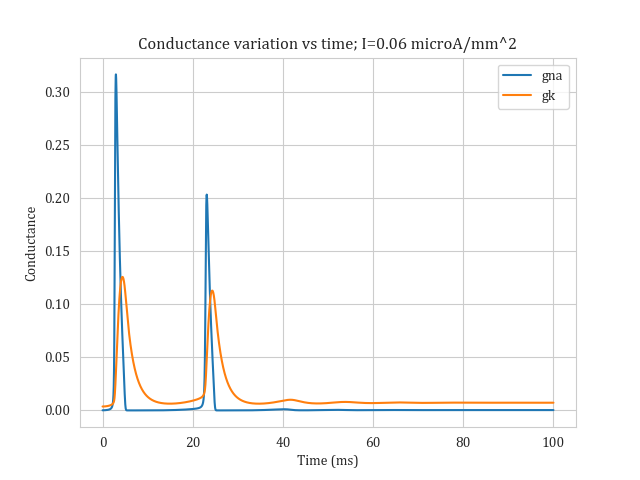
\includegraphics[scale=0.6]{images/finite_conductance.png}
	% 	\caption{Variation of Voltage, Gating variables and Conductance at current instant \tt{I2}. Finite number of voltage spikes are observed. Number of iterations performed: $10^4$}
	% \end{figure}

	% \begin{figure}[H]
	% 	\centering
	% 	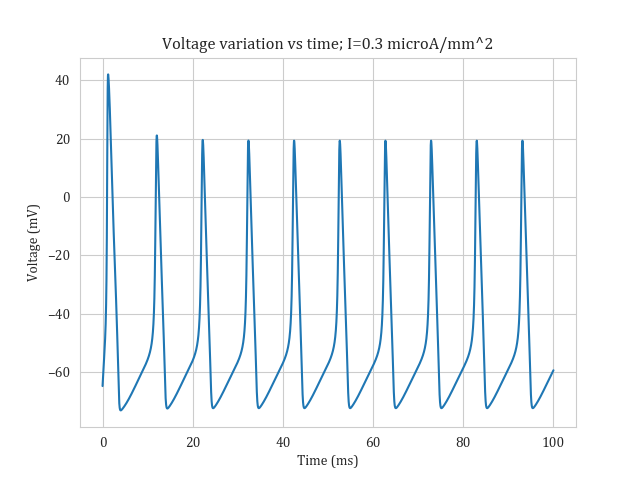
\includegraphics[scale=0.6]{images/large_i_v.png}
	% 	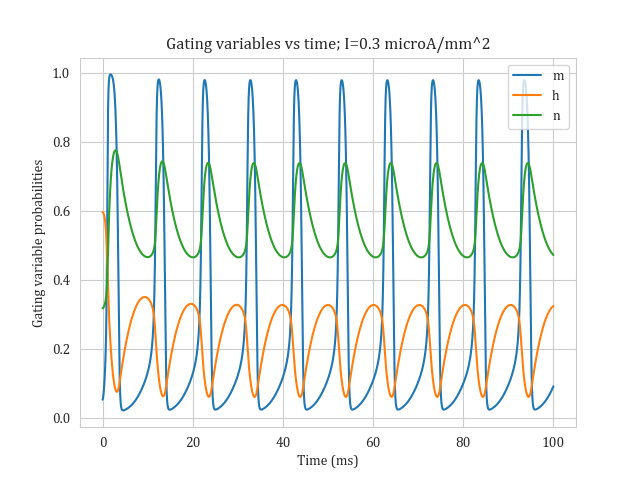
\includegraphics[scale=0.6]{images/large_i_gating.png}
	% 	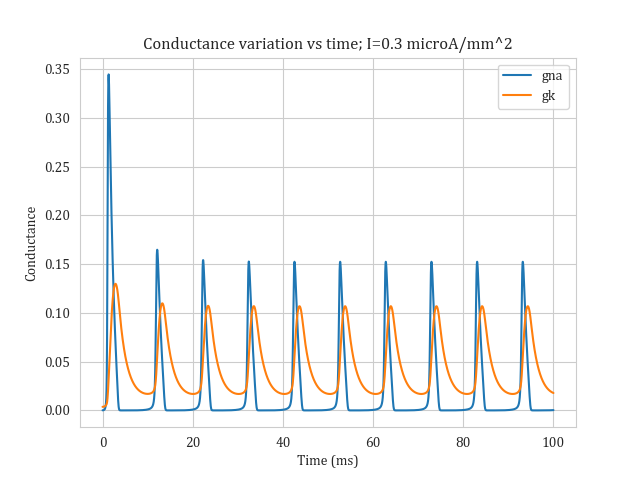
\includegraphics[scale=0.6]{images/large_i_conductance.png}
	% 	\caption{Variation of Voltage, Gating variables and Conductance at current instant \tt{I3}. Limit cycle behavior in voltage spikes is observed. Number of iterations performed: $10^4$}
	% \end{figure}

	% \begin{figure}[H]
	% 	\centering
	% 	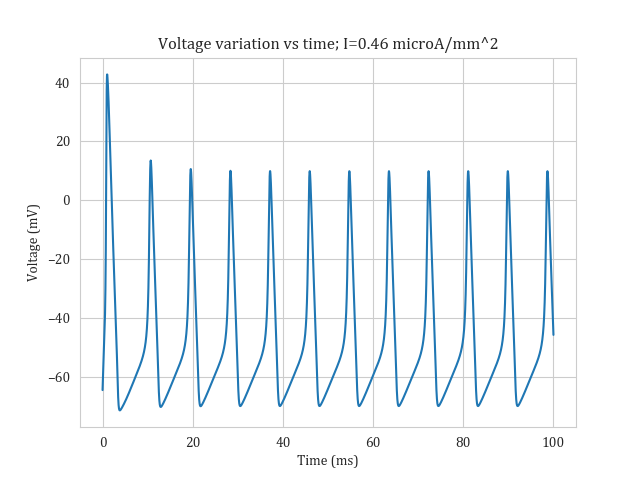
\includegraphics[scale=0.6]{images/vlarge_i_v.png}
	% 	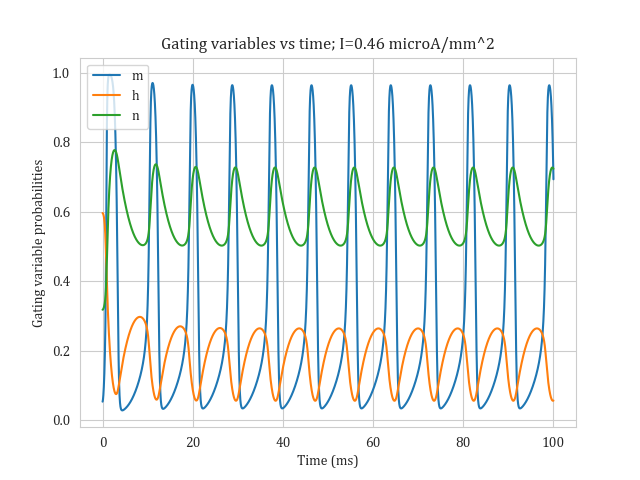
\includegraphics[scale=0.6]{images/vlarge_i_gating.png}
	% 	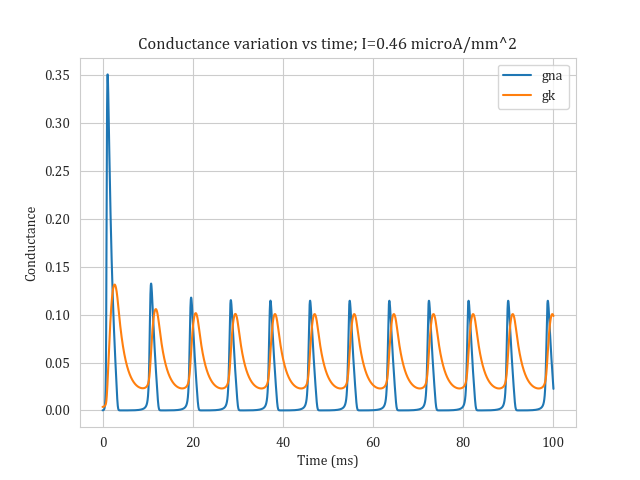
\includegraphics[scale=0.6]{images/vlarge_i_conductance.png}
	% 	\caption{Variation of Voltage, Gating variables and Conductance at current instant after \tt{I3}. Significant reduction in the number of spikes with amplitude greater than \tt{10mV} is observed. Number of iterations performed: $10^4$}
	% \end{figure}
\end{document}